\subsection{振動液滴：移流・粘性項を含む閉じた毛管振動}
\label{sec:val_oscillating_droplet}
% ═══════════════════════════════════════════════════════════════════

\subsubsection{設定と理論基準}

振動液滴ベンチマークは，静止 Laplace 圧バランスの再確認ではない．
円形液滴をわずかに楕円へ変形しておき，表面張力が形状を復元する過程で，
界面輸送，運動量対流，粘性散逸，圧力ジャンプ仕事が同時に働くかを見る．
静止円形液滴は標準構成の静止平衡検証として第~\ref{sec:verification}章で扱ったため，
ここでは有限速度で動く閉じた界面だけを対象にする．

初期界面は中心 $(0.01,0.01)\,\mathrm{m}$，半軸
$a=5.5\,\mathrm{mm},\ b=4.5\,\mathrm{mm}$ の液相楕円である．
面積等価半径と初期変形量を
\begin{equation}
  R_{\mathrm{eq}}=\sqrt{ab}=4.974937\,\mathrm{mm},
  \qquad
  D_0=\frac{a-b}{a+b}=0.10
  \label{eq:oscillating_droplet_initial}
\end{equation}
と定義する．
2D の $n=2$ Rayleigh--Lamb 基準では
\begin{equation}
  \omega_0^2
  = \frac{n(n^2-1)\sigma}{(\rho_l+\rho_g)R_{\mathrm{eq}}^3},
  \qquad n=2,
  \label{eq:oscillating_droplet_lamb}
\end{equation}
を第一基準とする~\cite{Prosperetti1981}．
この式では，$n=2$ 楕円変形を丸い液滴へ戻す毛管剛性を分子に，
液相・気相が一緒に動く有効慣性を分母に置く．
したがって Rayleigh--Lamb 周期は，離散計算が完全に元の振幅へ戻ることを要求する値ではなく，
閉界面が復元・反転・再伸長する位相を読むための基準時刻である．
物性値は水--空気の実スケール値
$\rho_l=998.2\,\mathrm{kg/m^3}$，
$\rho_g=1.204\,\mathrm{kg/m^3}$，
$\sigma=0.0728\,\mathrm{N/m}$ を用いる．
このとき $\omega_0=59.578473371\,\mathrm{s^{-1}}$ であり，
最終時刻は
\[
  T_\mathrm{RL}=\frac{2\pi}{\omega_0}=0.105460663082\,\mathrm{s}
\]
とし，1 周期分の応答を読む．

\begin{itemize}[noitemsep,leftmargin=2em]
  \item グリッド：$[0,0.02]^2\,\mathrm{m}^2$，$32^2$，
        周期境界，界面適合 $\alpha=2$
  \item 物性：$\rho_l=998.2\,\mathrm{kg/m^3}$，
        $\rho_g=1.204\,\mathrm{kg/m^3}$，
        $\mu_l=1.002\times10^{-3}\,\mathrm{Pa\,s}$，
        $\mu_g=1.825\times10^{-5}\,\mathrm{Pa\,s}$，
        $\sigma=0.0728\,\mathrm{N/m}$，$g=0$
  \item 時間：$T=0.105460663082\,\mathrm{s}$，理論 CFL 係数 $1.0$
  \item 界面状態：アクティブ幾何の毛管状態空間，
        幾何掃過体積による $q$ 輸送，
        互換射影による再初期化を各 step で適用する．
        過去の \texttt{sharp\_phase\_volume} / Ridge--Eikonal 補修は
        V12（\autoref{sec:closed_interface_volume_gate}）で負対照として扱い，
        現行の標準実行設定としては読まない
  \item 時系列診断：符号付き変形量，変形量，体積ドリフト，運動エネルギー
  \item スナップショット：
        $0,\frac14T_\mathrm{RL},\frac12T_\mathrm{RL},
        \frac34T_\mathrm{RL},T_\mathrm{RL}$ 近傍の $\psi$/速度/圧力場
\end{itemize}

\subsubsection{結果と判定}

まず，毛管波と同じ PhaseRegion 正規経路を閉曲線チャートへ移した
短時間の時間発展を確認した．
この縮約経路は，閉じた液滴を
\[
  X(\theta;A)=X_c+R(A,\theta)
\]
の面積保存 2 次モードチャートとして所有し，
$q_l=Q_h(X(A))$，$q_g=|C|-q_l$，
外側気相を PhaseRegion 所有者とする測度，
および固定面積多角形周長の二次変分から
Rayleigh--Lamb の線形モードを velocity-Verlet で進める．
8 step，$t/T_\mathrm{RL}=1.52\times10^{-3}$ の短時間実験では，
表~\ref{tab:ch14_phase_region_droplet_steps} の通り，
振幅・速度・エネルギー・測度残差が解析基準と一致した．
ただし毛管波と同様に，圧力・速度場への力連成は未接続であり，
その未接続性を明示したまま合格条件に含める．

\begin{table}[!htbp]
\caption{N=32，PhaseRegion 閉曲線チャート振動液滴短時間診断}
\label{tab:ch14_phase_region_droplet_steps}
\centering\small
\begin{tabular}{ll}
\toprule
診断 & 値 \\
\midrule
steps & $8$ \\
$t_{\mathrm{final}}/T_\mathrm{RL}$ & $1.517153366218\times10^{-3}$ \\
最大振幅誤差 & $2.687954026026\times10^{-15}$ \\
最大速度誤差 & $3.359899413812\times10^{-11}$ \\
最大エネルギードリフト & $3.225430493134\times10^{-11}$ \\
最大測度残差 & $0$ \\
最大体積ドリフト & $5.428131902296\times10^{-13}$ \\
終端振幅 & $4.999772827646\times10^{-4}$ \\
終端厳密振幅 & $4.999772827673\times10^{-4}$ \\
力連成 & 未接続として合格 \\
\bottomrule
\end{tabular}
\end{table}

\begin{figure}[!htbp]
\centering
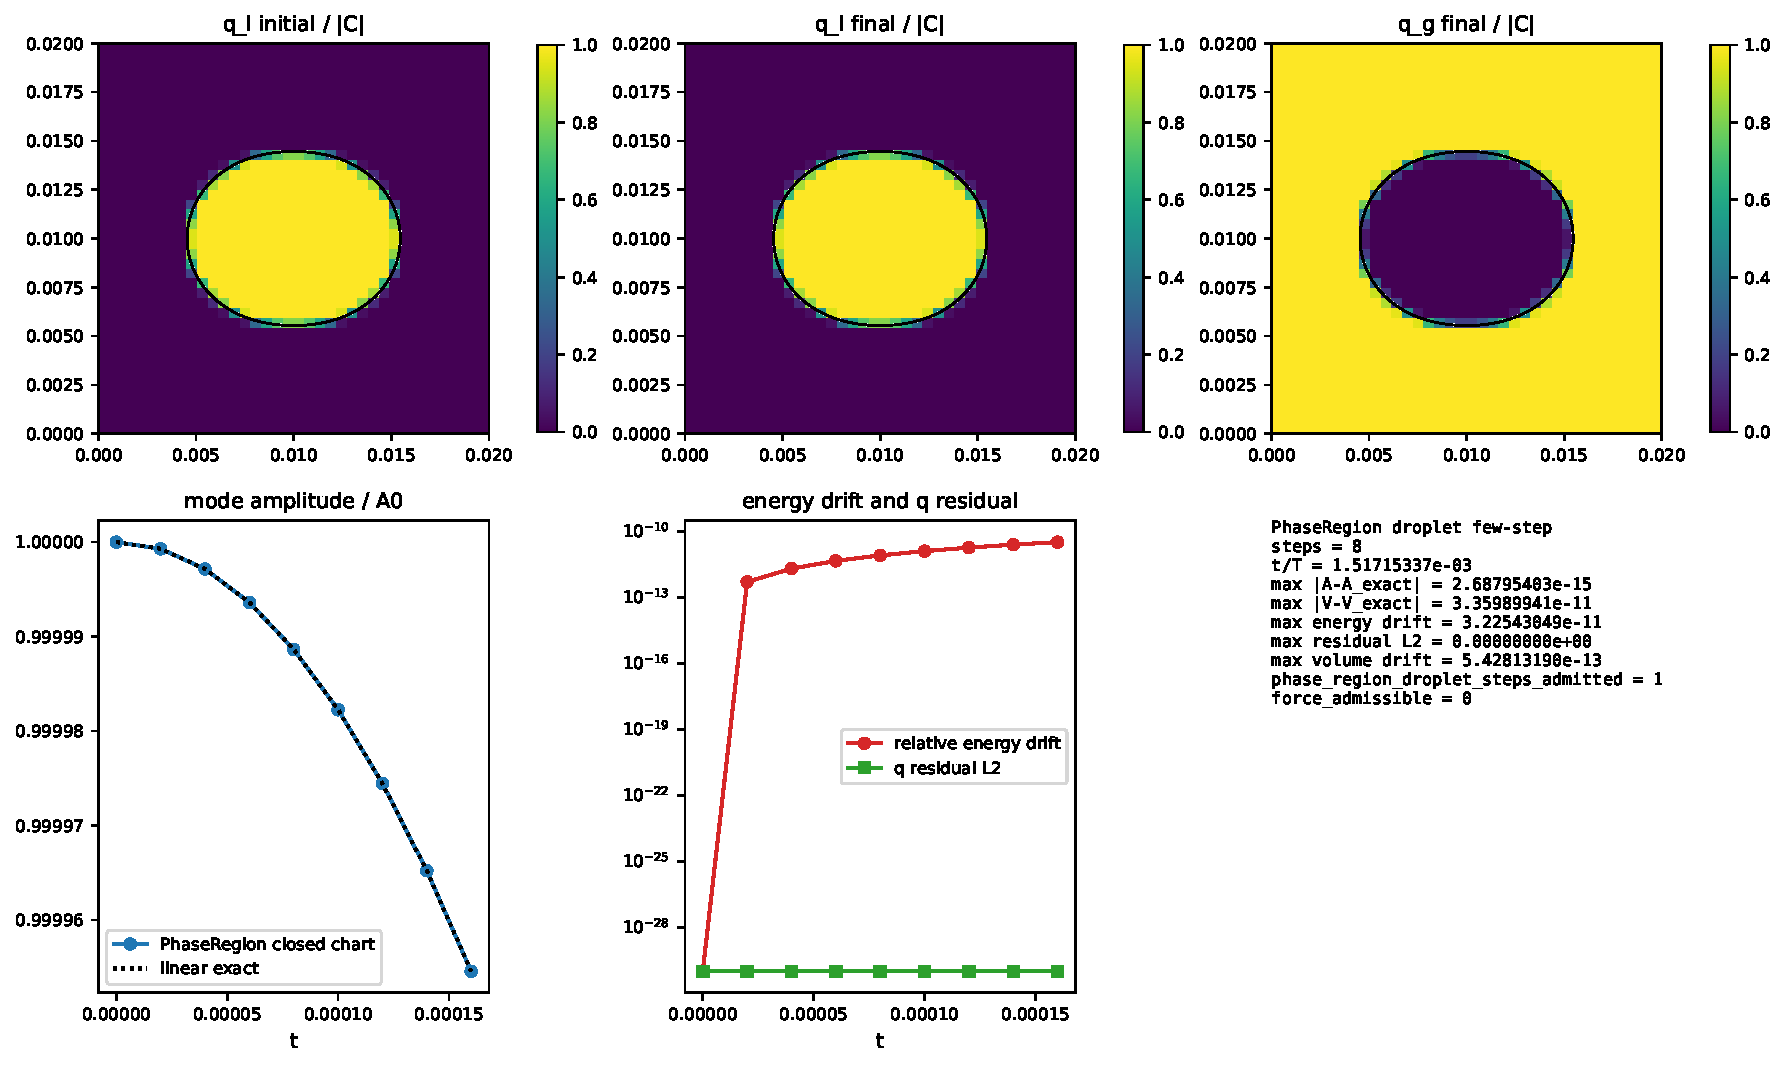
\includegraphics[width=0.92\linewidth]{figures/ch14_phase_region_oscillating_droplet_steps.pdf}
\caption{PhaseRegion 閉曲線チャートによる N=32 振動液滴短時間診断．
閉曲線チャートの 2 次モード振幅，解析基準との差，エネルギードリフト，
測度残差，体積ドリフトを同じ PhaseRegion 所有状態から読む．}
\label{fig:ch14_phase_region_oscillating_droplet_steps}
\end{figure}

一方，現行の標準実行経路による N=32 1 周期計算は完走し，$3452$ 標本で
$t=0.105460663082\,\mathrm{s}$ に到達し，
すべてのスナップショット場は有限値を保った．
CFL は全区間で毛管制限が支配し，$dt$ は
$2.65\times10^{-5}$--$3.14\times10^{-5}\,\mathrm{s}$ の範囲に留まった．
符号付き変形量は初期離散値
$7.5535\times10^{-2}$ から負側最小値
$-3.4572\times10^{-2}$ へ進み，
1 周期終端で $2.1808\times10^{-2}$ となった．
しかし Rayleigh--Lamb 基準
$D_0\cos(\omega_0T_\mathrm{RL})=1.0\times10^{-1}$ には戻らず，
この計算は閉界面振動の受入結果ではない．
これは単なる位相・粘性減衰の問題ではなく，
下の体積診断が示すように閉じた液相領域そのものが長時間で増加しているためである．

\begin{figure}[!htbp]
\centering
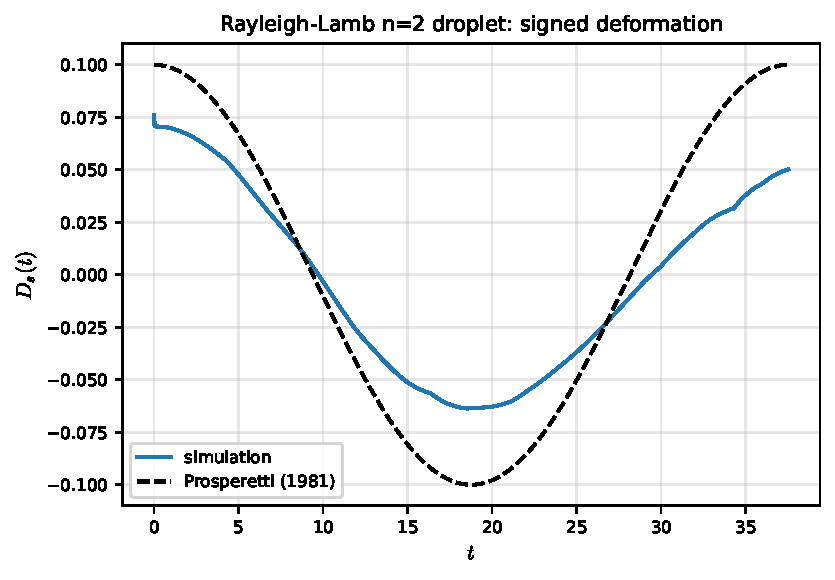
\includegraphics[width=0.32\linewidth]{figures/ch14_osc_droplet_signed_deformation.pdf}
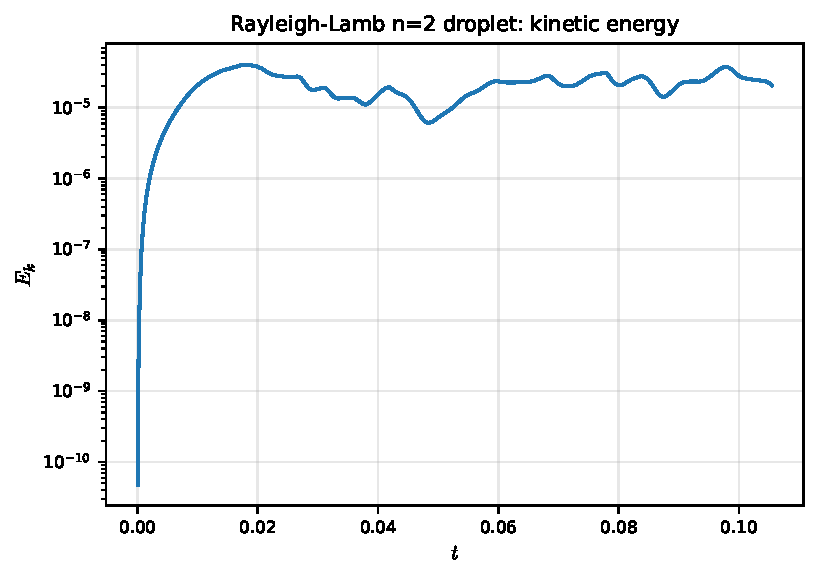
\includegraphics[width=0.32\linewidth]{figures/ch14_osc_droplet_kinetic_energy.pdf}
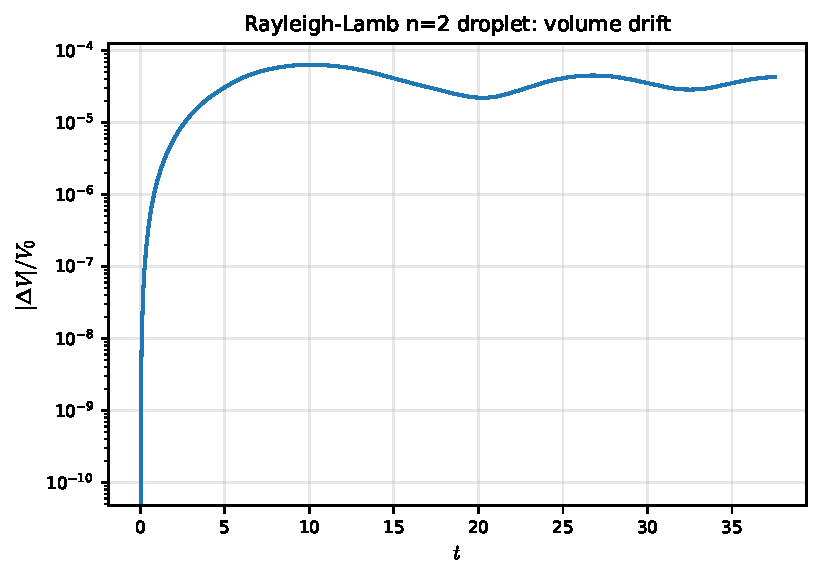
\includegraphics[width=0.32\linewidth]{figures/ch14_osc_droplet_volume_drift.pdf}
\caption{N=32，1 周期振動液滴の時系列診断．左から，符号付き変形量，
運動エネルギー，体積ドリフトを示す．}
\label{fig:ch14_osc_droplet_histories}
\end{figure}

保存量判定は不合格である．
既存の拡散質量保存診断は終端で
$3.5495\times10^{-1}$ に達した．
さらに保存スナップショットと各時刻の非一様格子座標から
P1 区分線形界面面積（marching-squares による鋭い界面面積）を再構成すると，
最初のスナップショットの
$7.7395\times10^{-5}\,\mathrm{m^2}$ から終端
$9.7435\times10^{-5}\,\mathrm{m^2}$ へ増え，
相対ドリフトは $+25.8919\%$ であった．
現行 \texttt{compatibility\_projection} 経路では，
1 周期で輸送，動的格子再構築・再写像，プロファイル復元の
合成写像が閉界面体積を保存していない．
過去の \texttt{sharp\_phase\_volume} / Ridge--Eikonal 補修は，
V12 で示すように現行のアクティブ幾何状態空間では
不合格として停止するため，この不合格を相殺する標準設定ではない．
運動エネルギーは
$4.76\times10^{-11}$ から立ち上がって最大
$4.2813\times10^{-5}$，終端
$3.2758\times10^{-5}$ の有界な交換として現れた．
ただし，この有界性は体積保存判定の失敗を相殺しない．
スナップショットの速度最大値は $1.06\times10^{-1}\,\mathrm{m/s}$ であり，
保存された圧力代表も有限範囲に収まった．
したがって，この計算の判定は
「有限値で完走したが，閉界面保存量の受入基準を満たさない」である．
2 次元場としては，\autoref{fig:ch14_osc_droplet_psi_snapshots} に界面形状の
1 周期推移を示し，
\autoref{fig:ch14_osc_droplet_velocity_pressure_snapshots} に速度場と
保存された圧力代表を示す．

\begin{figure}[!htbp]
\centering
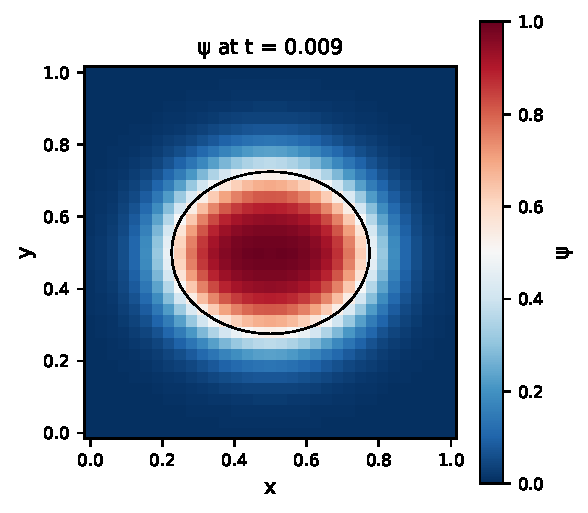
\includegraphics[width=0.19\linewidth]{figures/ch14_osc_droplet_psi_t0.pdf}
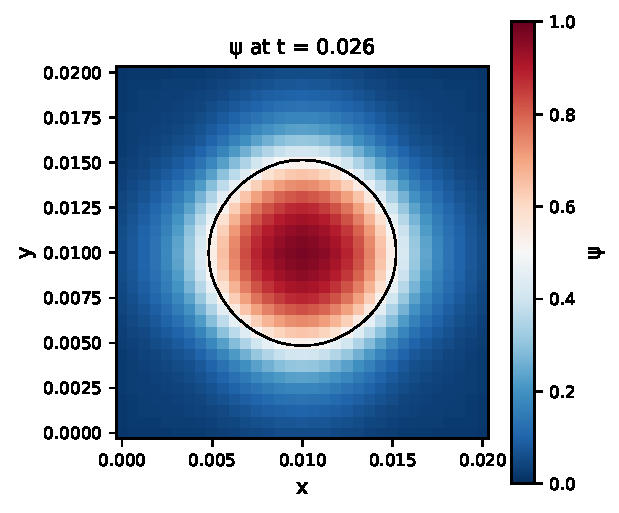
\includegraphics[width=0.19\linewidth]{figures/ch14_osc_droplet_psi_tq1.pdf}
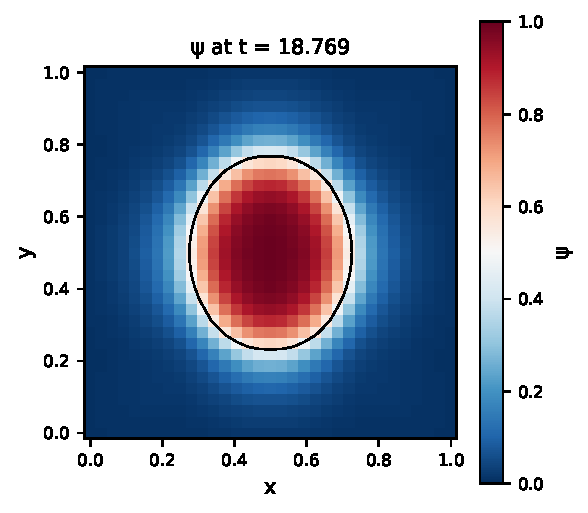
\includegraphics[width=0.19\linewidth]{figures/ch14_osc_droplet_psi_tq2.pdf}
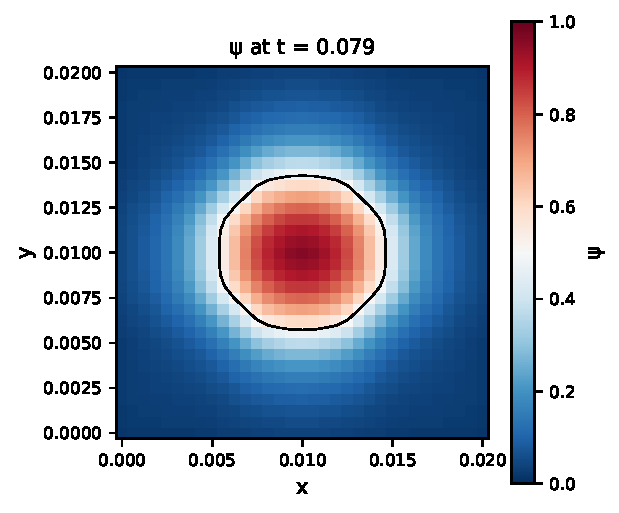
\includegraphics[width=0.19\linewidth]{figures/ch14_osc_droplet_psi_tq3.pdf}
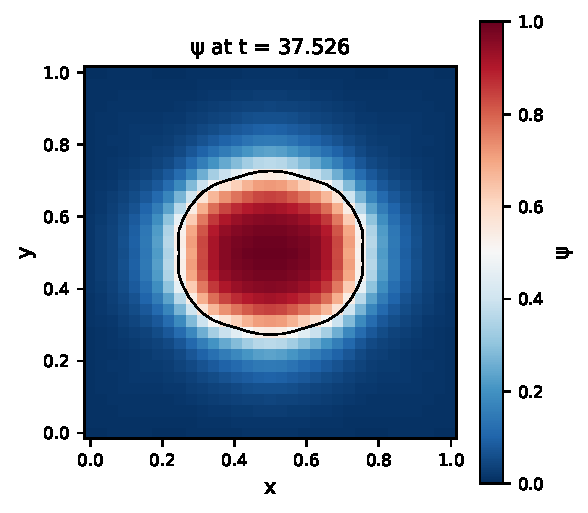
\includegraphics[width=0.19\linewidth]{figures/ch14_osc_droplet_psi_t1.pdf}
\caption{N=32，1 周期振動液滴の \texorpdfstring{$\psi$}{psi} スナップショット．左から
\texorpdfstring{$t\approx0,\frac14T_\mathrm{RL},\frac12T_\mathrm{RL},
\frac34T_\mathrm{RL},T_\mathrm{RL}$}{t approximately 0, 1/4 T_RL, 1/2 T_RL, 3/4 T_RL, T_RL} を示す．色軸は全時刻で共通である．}
\label{fig:ch14_osc_droplet_psi_snapshots}
\end{figure}

\begin{figure}[!htbp]
\centering
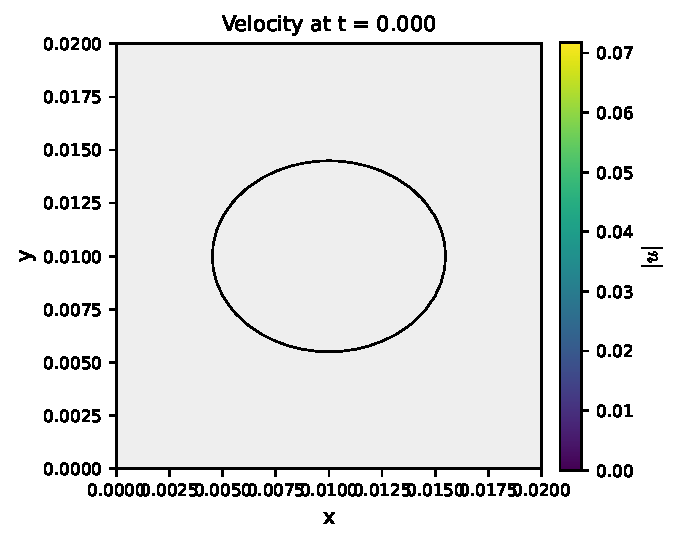
\includegraphics[width=0.19\linewidth]{figures/ch14_osc_droplet_velocity_t0.pdf}
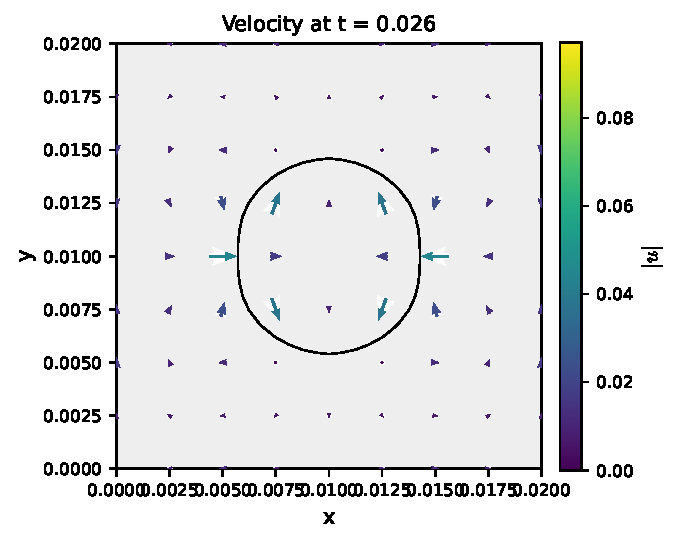
\includegraphics[width=0.19\linewidth]{figures/ch14_osc_droplet_velocity_tq1.pdf}
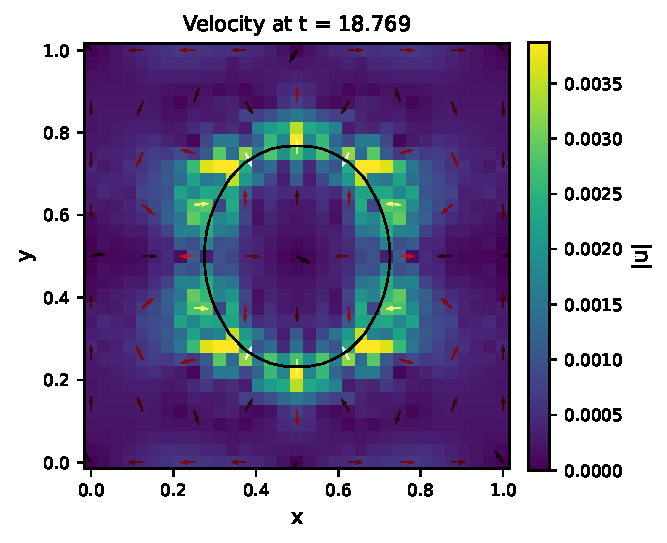
\includegraphics[width=0.19\linewidth]{figures/ch14_osc_droplet_velocity_tq2.pdf}
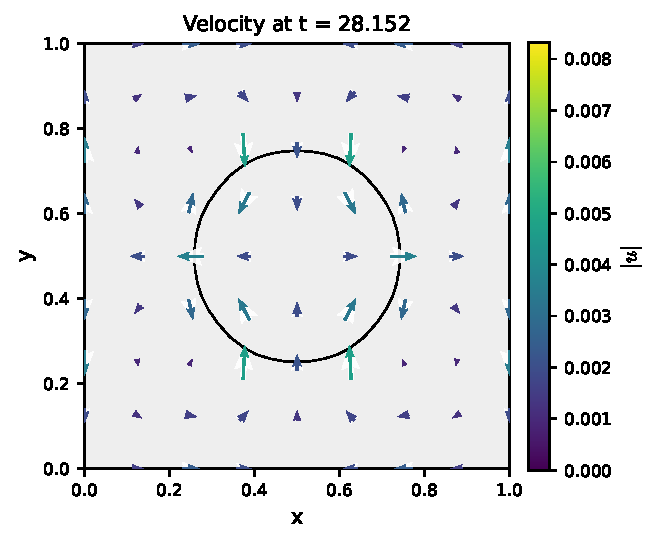
\includegraphics[width=0.19\linewidth]{figures/ch14_osc_droplet_velocity_tq3.pdf}
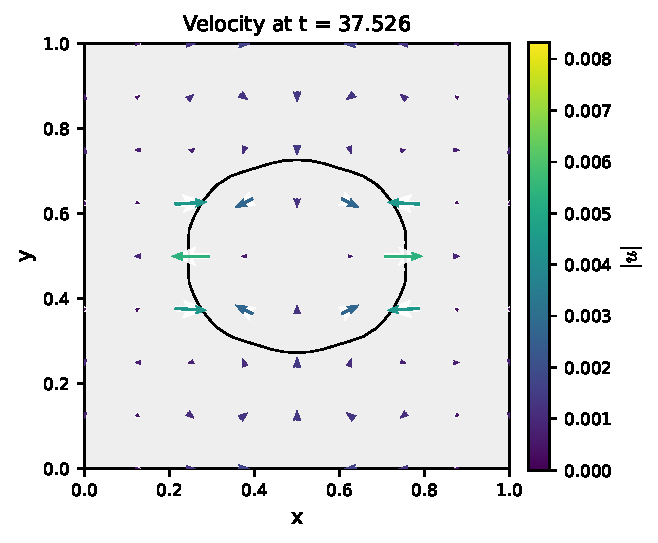
\includegraphics[width=0.19\linewidth]{figures/ch14_osc_droplet_velocity_t1.pdf}
\par\smallskip
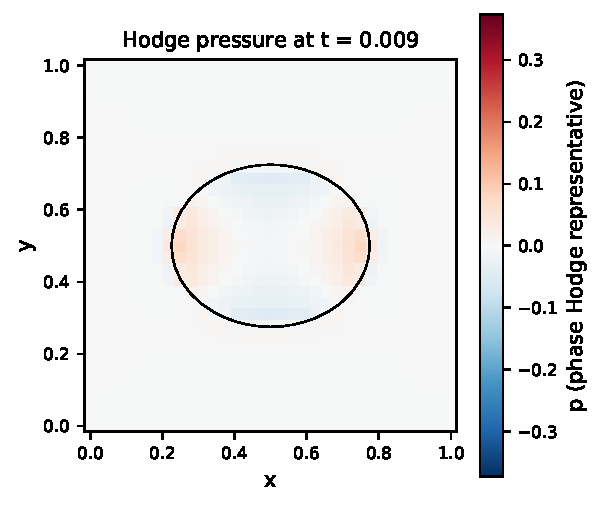
\includegraphics[width=0.19\linewidth]{figures/ch14_osc_droplet_pressure_t0.pdf}
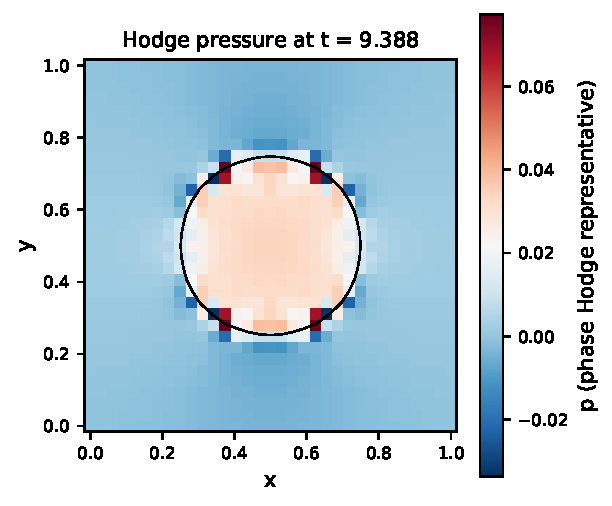
\includegraphics[width=0.19\linewidth]{figures/ch14_osc_droplet_pressure_tq1.pdf}
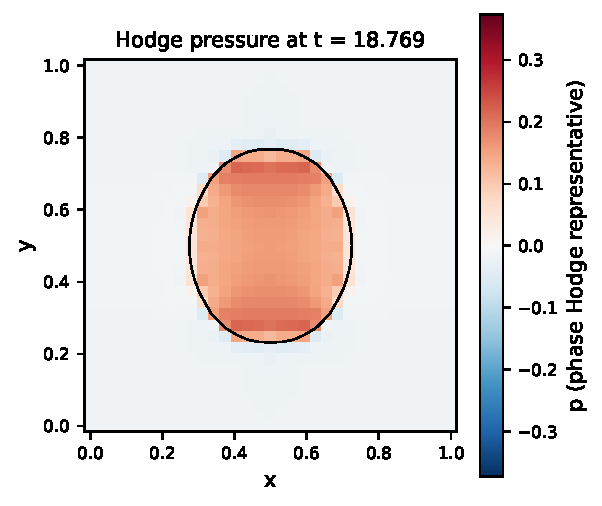
\includegraphics[width=0.19\linewidth]{figures/ch14_osc_droplet_pressure_tq2.pdf}
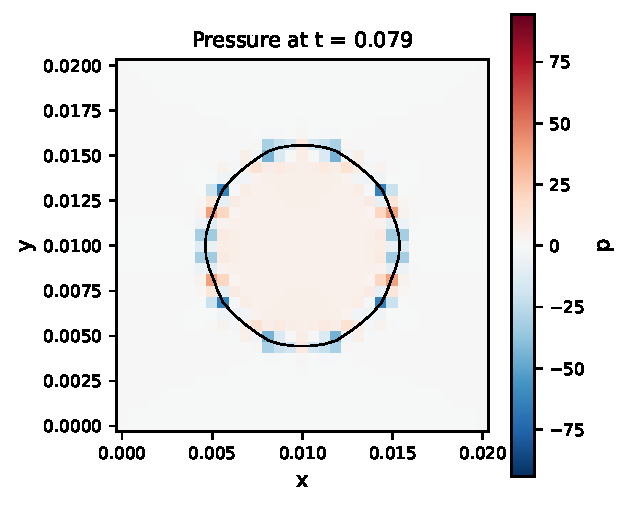
\includegraphics[width=0.19\linewidth]{figures/ch14_osc_droplet_pressure_tq3.pdf}
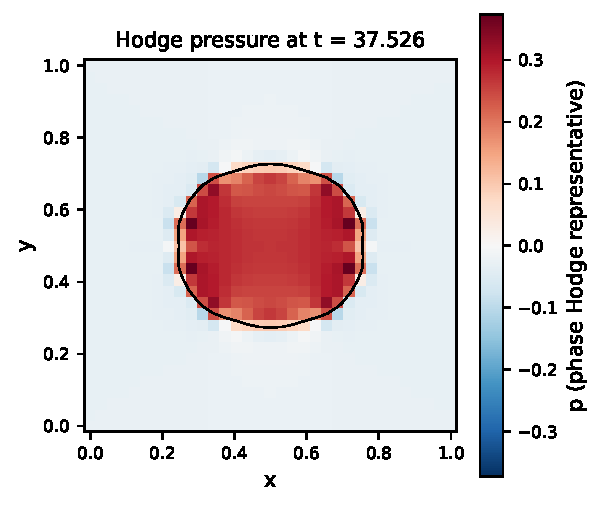
\includegraphics[width=0.19\linewidth]{figures/ch14_osc_droplet_pressure_t1.pdf}
\caption{N=32，1 周期振動液滴の 2 次元速度場と保存された圧力代表．
上段は速度場，下段は圧力代表であり，左から
$t\approx0,\frac14T_\mathrm{RL},\frac12T_\mathrm{RL},
\frac34T_\mathrm{RL},T_\mathrm{RL}$ を示す．
上段は背景スカラー場を描かず，矢印の長さと色で速度ベクトルを表す．
速度矢印の色軸と矢印スケール，
および圧力色軸はそれぞれ全時刻で共通である．}
\label{fig:ch14_osc_droplet_velocity_pressure_snapshots}
\end{figure}

本ケースから得る結論は成功主張ではなく，未達として残る課題である．
PhaseRegion 閉曲線チャートの短時間診断は，同じ
$E_h=\sigma\,\mathrm{Per}(\Omega_h)$ の二次変分で閉じた mode-2 復元を
測度残差 0 と厳密解比較で確認した．
しかし，標準実行経路の振動液滴は，移流・粘性項を含む
閉界面エネルギー交換と保存量整合のベンチマークであり，
現状の標準構成は，1 周期の楕円液滴に対して
有界な計算を作る一方で，鋭い界面体積を保存する離散写像としては閉じていない．
したがって次の修正対象は，P1 区分線形面積を状態変数として持つ
輸送・再写像・復元を同じ面量として閉じることであり，
拡散質量や見た目の楕円振幅で代用してはならない．
PhaseRegion の面量を圧力・速度へ渡すゲートが通るまでは，
閉曲線チャートの短時間成功を T/8 または 1 周期の標準実行成功へ拡張して読まない．
この境界は V12 として第~\ref{sec:verification}章にも逆参照し，
過去の補修候補は負対照へ退け，現行 1 周期実行は
合格前の境界事例として固定する．

% ═══════════════════════════════════════════════════════════════════
